\mainmatter%
\setcounter{page}{1}

\lectureseries[\course]{\course}

\auth[\lecAuth]{Lecturer: \lecAuth\\ Scribe: \scribe}
\date{February 4, 2010}

\setaddress%

% the following hack starts the lecture numbering at 1
\setcounter{lecture}{9}
\setcounter{chapter}{9}

\lecture{Stability \& Instability}

\section{Global Asymptotic Stability}
To obtain global asymptotic stability it is not enough for the Lyapunov function $V$ to be positive definite.

\begin{example}
Let the Lyapunov function be

\begin{equation*}
V = \frac{x_1^2}{1+x_1^2} + x_2^2.
\end{equation*}

This function is positive definite.
Notice that the first term is bounded but not the second term.
This leads to level sets that look like those in Figure~\ref{fig:10levelSets}.
With such level sets it is possible to move in the negative direction but the states ($x_1$) could be going to infinity.
$\lozenge$
\end{example}

\begin{figure}[ht!]
\centering
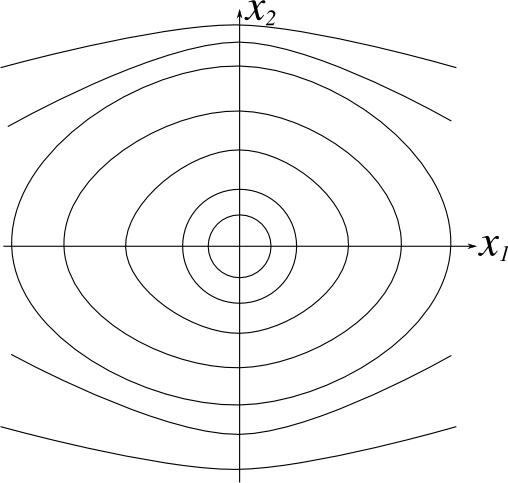
\includegraphics[width=.4\textwidth]{images/10levelSets}
\caption{Level sets.}%
\label{fig:10levelSets}
\end{figure}

For global asymptotic stability it is necessary for the level sets to be bounded.

\begin{definition}
$V(x)$ is \textit{radially unbounded} if $V(x)\to\infty$ as $|x|\to\infty$.
\end{definition}

\begin{theorem}{Global Asymptotic Stability}
If the Lyapunov function $V$ is positive definite and radially unbounded and $\dot{V}$ is negative definite then the equilibrium point $x=0$ has global asymptotic stability.
\end{theorem}

\begin{example}
Let the system be defined by
\begin{align*}
\dot{x}_1 &= -x_1 + x_2^3 \\
\dot{x}_2 &= -x_1 - x_2.
\end{align*}
Try the Lyapunov function

\begin{equation*}
V = \frac{x_1^2}{2} + \frac{x_2^2}{4}.
\end{equation*}

Taking the derivative yields

\begin{equation*}
\dot{V} = -x_1^2 - x_2^2
\end{equation*}

which is negative definite and implies that the equilibrium point $x=0$ has global asymptotic stability.
$\lozenge$
\end{example}

\section{Completion of Squares}
In general completion of squares is given by

\begin{equation*}
a^T b \leq \tfrac{1}{2}|a|^2 + \tfrac{1}{2}|b|^2
\end{equation*}

In the scalar case we have

\begin{equation*}
{(a-b)}^2 = a^2 - 2ab + b^2 \geq 0.
\end{equation*}

\begin{example}
Let the system be
\begin{align*}
\dot{x}_1 &= -x_1 + x_2 \\
\dot{x}_2 &= -x_2.
\end{align*}
Let the Lyapunov function be

\begin{equation*}
V = \frac{x_1^2+x_2^2}{2}.
\end{equation*}

Then the derivative is

\begin{equation*}
\dot{V} = x_1\dot{x}_1 + x_2\dot{x}_2 = -x_1^2 - x_2^2 + x_1x_2.
\end{equation*}

By completion of squares this leads to

\begin{equation*}
x_1x_2 \leq \tfrac{1}{2}x_1^2 + \tfrac{1}{2}x_2^2
\end{equation*}

which implies that $\dot{V} \leq V$.
Since $V \geq 0$ this means that $\dot{V} \leq 0$.
$\lozenge$
\end{example}

\section{Instability}
\begin{example}
Two different unstable second order systems are shown in Figure~\ref{fig:10instability}.
$\lozenge$
\end{example}

\begin{figure}[ht!]
\centering
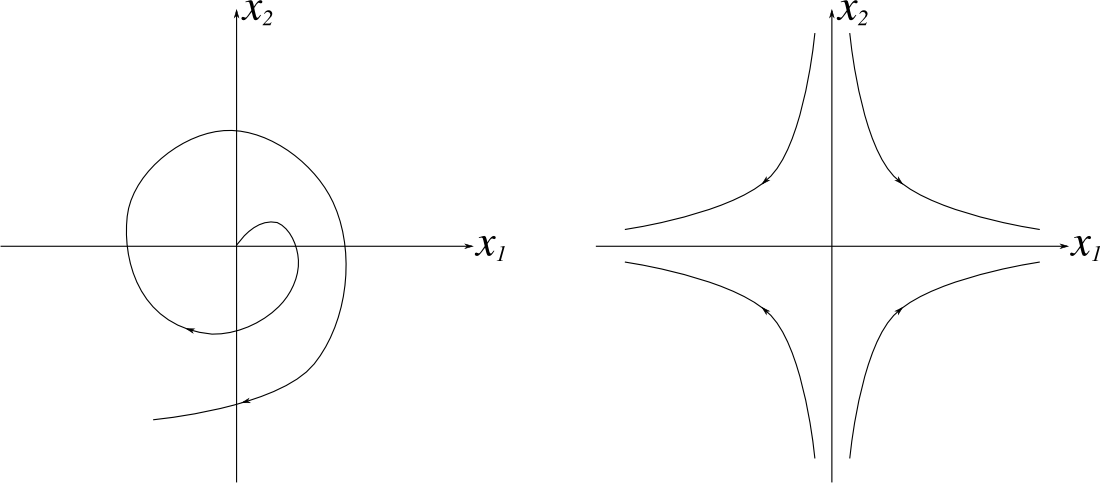
\includegraphics[width=.4\textwidth]{images/10instability}
\caption{Unstable second order systems.}%
\label{fig:10instability}
\end{figure}

\begin{theorem}%
\label{th:instability}
Let $x=0$ be an equilibrium point of $\dot{x}=f(t,x)$.
Let $V:\mathcal{D}\to\mathbb{R}$, $V\in\mathcal{C}^1$, $V(0)=0$ and $V(x_0)>0$ for some arbitrarirly small $|x_0|$.
Define $\mathcal{U}=\{x\in \mathcal{B}_r | V(x)>0\}$ and suppose that $\dot{V}>0 \forall x\in\mathcal{U}$.
Then $x=0$ is unstable.
\end{theorem}

Figure~\ref{fig:10theoremBall} helps with the concept of instability as defined by Theorem~\ref{th:instability}.
The condition $\dot{V}>0\forall x\in\mathcal{U}$ means that $V$ \textit{cannot} decrease in the space $\mathcal{U}$.
All trajectories in $\mathcal{U}$ must exit through the boundary of $\mathcal{U}$, $\partial\mathcal{U}$.
A system is considered unstable when escape routes exist for some of the trajectories as that is when certain states ``blow up''.

\begin{figure}[ht!]
\centering
\includegraphics[width=.4\textwidth]{images/10theoremBall}
\caption{Instability theory.}%
\label{fig:10theoremBall}
\end{figure}

\begin{example}
Let the system be
\begin{align*}
\dot{x}_1 &= x_1 \\
\dot{x}_2 &= -x_2.
\end{align*}
Try the Lyapunov function and derivative
\begin{align*}
V &= \frac{x_1^2}{2} - \frac{x_2^2}{2} \\
\dot{V} &= x_1^2 + x_2^2.
\end{align*}
This shows that $V>0$ and $\dot{V}>0\in\mathcal{U}$ so we satisfy Chataev's theorem and the system is unstable.
See Figure~\ref{fig:10unstableV}.
$\lozenge$
\end{example}

\begin{figure}[ht!]
\centering

\includegraphics[width=.4\textwidth]{images/10unstableV}
\caption{Instability regions.}%
\label{fig:10unstableV}
\end{figure}

\begin{example}
Let the system dynamics, motivated by adaptive control theory, be given by
\begin{align*}
\dot{x} &= |x|x + (1+|x|)xy \\
\dot{y} &= -\tfrac{1}{8}(1+|x|)x^2.
\end{align*}
Let the first attempt be with
\begin{align*}
V &= x^2 + 8y^2 \\
\dot{V} &= 2|x|^3
\end{align*}
where $V$ is positive definite and $\dot{V}$ is positive semidefinite.
Then $\mathcal{U} = \{\mathbb{R}^2 - \{0,0\}\}$.
We can see that $\dot{V} = 0$ on the $y$-axis.

For the second attempt let $W=x^2-4y^2$ since the quadratic term $|x|x$ is the likely place for instabilities to occur because the cross terms are not anti-dissipative.
This leads to

\begin{equation*}
\mathcal{U} = \{|x|>2|y|\}
\end{equation*}

and the derivative of $W$ is

\begin{equation*}
\dot{W} = 2|x|^3 + 2(1+|x|)yx^2 + (1+|x|)yx^2.
\end{equation*}

Then we can look at the intersection of $\mathcal{U}$ with a circle of radius $\tfrac{1}{12}$ as in Figure~\ref{fig:10unstableW} and see that

\begin{equation*}
\dot{W} \geq \tfrac{1}{4}|x|^3 + \tfrac{3}{2}\underbrace{(|x|-2|y|)}_{>0\text{\ on\ }\mathcal{U}} + \tfrac{1}{4}|x|^3
\underbrace{(1-12\sqrt{x^2+y^2})}_{>0\text{\ on\ }\mathcal{B}_{1/12}}.
\end{equation*}

This shows that $\dot{W}>0$ on $\mathcal{U}\cap\mathcal{B}_{1/12}$ and leads to the conclusion that $x=y=0$ is unstable.
$\lozenge$
\end{example}

\begin{figure}[ht!]
\centering
\includegraphics[width=.4\textwidth]{images/10unstableW}
\caption{Intersection of instability regions.}%
\label{fig:10unstableW}
\end{figure}
